\subsection*{Interfejs użytkownika}
Przygotowano prosty interfejs w bibliotece Streamlit (\texttt{app.py}, uruchomienie:
\texttt{streamlit run app.py}). Użytkownik wybiera model (domyślnie ResNet50 po strojeniu),
wgrywa obraz MRI (JPG/PNG) lub wybiera obraz z katalogu \texttt{Testing}, a aplikacja pokazuje:
\begin{itemize}
\item przewidzianą klasę i jej prawdopodobieństwo,
\item obraz wejściowy po przetworzeniu (skala szarości, 224$\times$224) obok mapy Grad-CAM,
\item wykres prawdopodobieństw wszystkich czterech klas.
\end{itemize}
Na górze strony jest wyraźne zastrzeżenie, że to narzędzie edukacyjne, a nie wyrób medyczny.
Pod mapą jest też informacja, że Grad-CAM nie jest segmentacją guza. Interfejs korzysta z tych
samych funkcji co notatniki (\texttt{load\_image}, \texttt{grad\_cam}), więc przetwarzanie
obrazu jest identyczne jak podczas ewaluacji. Rys.~\ref{fig:gui} pokazuje poprawną predykcję
guza przysadki oraz typowy błąd: glejak w sekwencji FLAIR rozpoznany z pełną pewnością jako
oponiak, mimo że mapa wskazuje guz.

\begin{figure}[H]
\centering
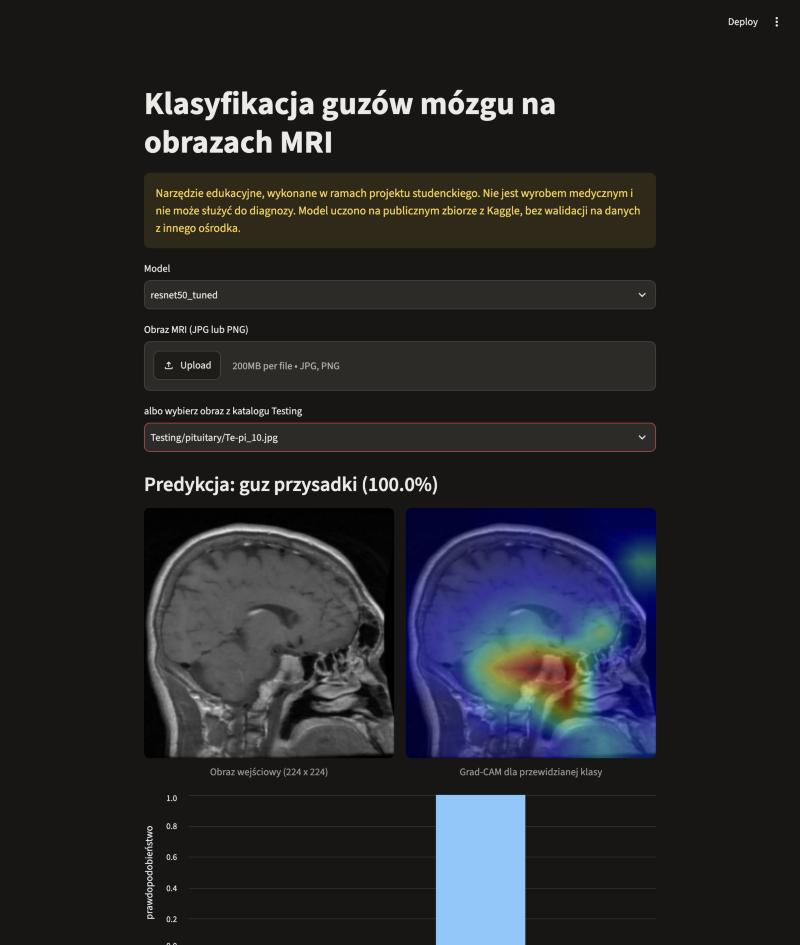
\includegraphics[width=0.48\linewidth]{gui_przysadka.jpg}\hfill
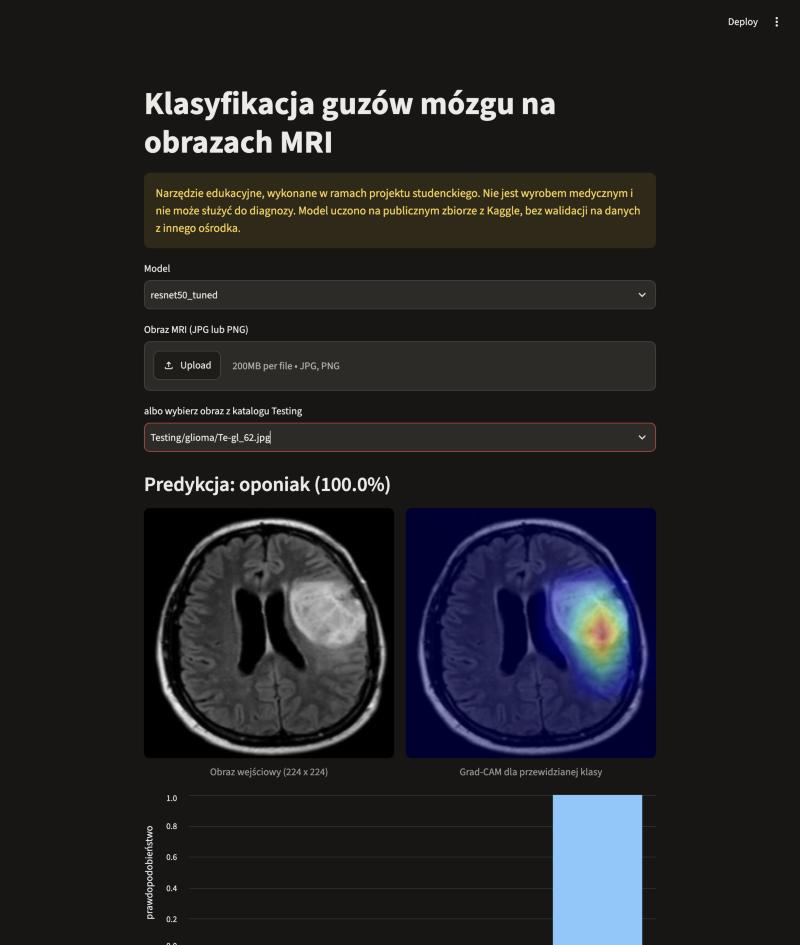
\includegraphics[width=0.48\linewidth]{gui_glejak_blad.jpg}
\caption{Interfejs Streamlit: poprawna predykcja guza przysadki (po lewej) i błędna predykcja
glejaka z innego źródła danych (po prawej).}
\label{fig:gui}
\end{figure}
